\documentclass{standalone}
\usepackage{tikz}
\usepackage{ctex,siunitx}
\usepackage{tkz-euclide}
\usepackage{amsmath}
\usetikzlibrary{patterns, calc}
\usetikzlibrary {decorations.pathmorphing, decorations.pathreplacing, decorations.shapes,}
\begin{document}
\small
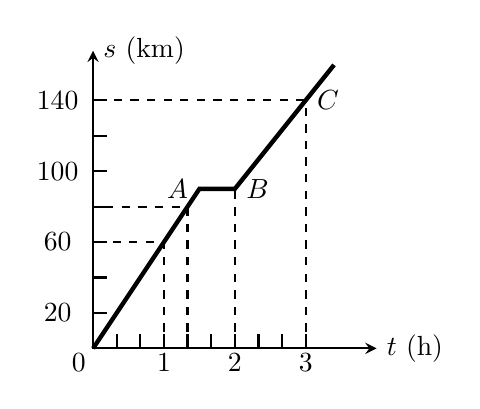
\begin{tikzpicture}[>=stealth, thick,scale=0.9]
  \draw [<->](0,4.2)node[right]{$s$ (\unit{km})}--(0,0)--(4,0)node[right]{$t$ (\unit{h})};
  \foreach \x in {1,2,3,...,9}
  {
      \draw(\x/3, 0) --(\x/3, .2);
  }
  \foreach \y in {1,2,3,...,7}
  {
      \draw(0,\y/2)--(.2, \y/2);
  }
  \node at (-.2,-.2){$0$};
  \node at (1,-.2){$1$};
  \node at (2,-.2){$2$};
  \node at (3,-.2){$3$};
  \node at (-.5,.5){$20$};
  \node at (-.5,1.5){$60$};
  \node at (-.5,2.5){$100$};
  \node at (-.5,3.5){$140$};
  \draw [dashed] (1,0)--(1,1.5)--(0,1.5);
  \draw [dashed] (1+1/3,0)--(1+1/3,2)--(0,2);
  \draw [dashed] (3,0)--(3,3.5)--(0,3.5);
  \draw [dashed] (2,0)--(2,2.25);
  \draw[ultra thick](0,0)--(1.5 ,2.25)node[left]{$A$}--(2,2.25)node[right]{$B$}--(3,3.5)node[right]{$C$}--(3.4,4.0);
  % \draw[ultra thick](2,2.25)node[right]{$B$}--(1.5 ,2.25)node[left]{$A$};
  % \draw[ultra thick](2,2.25)--(3,3.5)node[right]{$C$}--(4,4.75);
\end{tikzpicture}
\end{document}